\documentclass[a4paper,11pt]{article}

%%%%%%%%%
%%usees%%
%%%%%%%%%
\usepackage[utf8]{inputenc}
%\usepackage[ngerman]{babel}
%\usepackage{a4wide}
\usepackage[margin=3.0cm, top=3.0cm, bottom=3.0cm]{geometry}
\usepackage{setspace}
\usepackage{graphicx}
\usepackage{amssymb} 
\usepackage{amsmath}
\usepackage{mathtools}
\usepackage{footnote}
\usepackage{caption}
\usepackage{color}
\usepackage[hidelinks]{hyperref}
\usepackage{cite}
\usepackage{todonotes}
\usepackage{subcaption}
\usepackage{siunitx}
\usepackage{tabularx}
\usepackage{wrapfig}
\usepackage{url}
\usepackage{listings}


\newcommand{\reffig}[1]{Figure~\ref{#1}}
\newcommand{\refsec}[1]{Section~\ref{#1}}
\newcommand{\refdef}[1]{Definition~\ref{#1}}
\newcommand{\reflst}[1]{Listing~\ref{#1}}
\newcommand{\reftab}[1]{Table~\ref{#1}}

\definecolor{Mulberry}{cmyk}{0.34,0.90,0,0.02}
\definecolor{BrickRed}{cmyk}{0,0.89,0.94,0.28}
\lstset{language=C++,frame=none, basicstyle=\tt}
% \lstdefinelanguage{Lua}
% {
%   morekeywords={and,break,do,else,elseif,end,false,for,function,
%                 if,in,local,nil,not,or,repeat,return,then,true,until,while},
%   sensitive=true,
%   morecomment=[l]{--},
%   morecomment=[s]{--[[}{--]]},
%   morestring=[b]{"},
%   morestring=[s]{[==[}{]==]},
% }

% default style
\lstdefinestyle{Cpp}
{
  language=C++,
  basicstyle=\ttfamily,
  breaklines=true,
  showstringspaces=false,
  %keywordstyle=\bfseries,
  keywordstyle=\color{Mulberry},
  frame=lines,
  %belowcaptionskip=8pt,
  emphstyle=\itshape,
  %numbers=left,
  stepnumber=1,
  backgroundcolor=\color{blue!10},
  rulecolor=\color{blue!50},
  fillcolor=\color{blue!20},
  framexleftmargin=18pt,
  xleftmargin=18pt,
  % stringstyle=\color{BitterSweet},
  stringstyle=\color{BrickRed},
  commentstyle=\color{BrickRed},
  % emph={getup, servo, depends_skills},
  %emphstyle=\underbar,
  %numbers=left,
  %stepnumber=1,
  %%stringstyle=\ttfamily, % typewriter type for strings
  captionpos=b
}
\lstdefinestyle{SmallCpp}{
  style=Cpp,
  basicstyle=\ttfamily\footnotesize,
  numbersep=6pt,
}
\lstdefinestyle{ReallySmallCpp}{
  style=Cpp,
  basicstyle=\ttfamily\tiny,
  numbersep=5pt,
}

\definecolor{dkgreen}{rgb}{0,0.6,0}
\definecolor{gray}{rgb}{0.5,0.5,0.5}
\definecolor{mauve}{rgb}{0.58,0,0.82}
\definecolor{gray}{rgb}{0.4,0.4,0.4}
\definecolor{darkblue}{rgb}{0.0,0.0,0.6}
\definecolor{lightblue}{rgb}{0.0,0.0,0.9}
\definecolor{cyan}{rgb}{0.0,0.6,0.6}
\definecolor{darkred}{rgb}{0.6,0.0,0.0}


\lstdefinelanguage{XML}
{
  basicstyle=\ttfamily\footnotesize,
  columns=fullflexible,
  showstringspaces=false,
  numbers=left,                   % where to put the line-numbers
  numberstyle=\tiny\color{gray},  % the style that is used for the line-numbers
  stepnumber=1,
  numbersep=5pt,                  % how far the line-numbers are from the code
  backgroundcolor=\color{white},      % choose the background color. You must add \usepackage{color}
  showspaces=false,               % show spaces adding particular underscores
  showstringspaces=false,         % underline spaces within strings
  showtabs=false,                 % show tabs within strings adding particular underscores
  frame=none,                   % adds a frame around the code
  rulecolor=\color{black},        % if not set, the frame-color may be changed on line-breaks within not-black text (e.g. commens (green here))
  tabsize=2,                      % sets default tabsize to 2 spaces
  captionpos=b,                   % sets the caption-position to bottom
  breaklines=true,                % sets automatic line breaking
  breakatwhitespace=false,        % sets if automatic breaks should only happen at whitespace
  title=\lstname,                   % show the filename of files included with \lstinputlisting;
                                  % also try caption instead of title  
  commentstyle=\color{gray}\upshape,
  morestring=[s][\color{mauve}]{"}{"},
  morestring=[s][\color{black}]{>}{<},
  morecomment=[s]{<?}{?>},
  morecomment=[s][\color{dkgreen}]{<!--}{-->},
  stringstyle=\color{black},
  identifierstyle=\color{lightblue},
  keywordstyle=\color{red},
  morekeywords={xmlns,xsi,noNamespaceSchemaLocation,type,id,x,y,source,target,version,tool,transRef,roleRef,objective,eventually},
  basicstyle=\ttfamily\scriptsize,
  backgroundcolor=\color{blue!10},
  numbers=none,
  numbersep=5pt
}


\newcommand*\colvec[3][]{
    \begin{pmatrix}\ifx\relax#1\relax\else#1\\\fi#2\\#3\end{pmatrix}
}

%%%%%%%%%
%%Title%%
%%%%%%%%%

\author{Frederik Zwilling} \title{Solution Assesment Task: Four-Wheeled Robot}
\begin{document}
\maketitle
%%%%%%%%%
%%Text%%
%%%%%%%%

\textbf{Assessment:} You have been assigned the task of developing a
simple controller for a planar four-wheeled mobile robot that would
enable it to autonomously navigate around its environment. In order to
accomplish the forenamed objective, the following constituent
sub-tasks have been assigned:

\section{Configuration Kinematic Model}
\label{sec:e1}
\textbf{Task:} Derive the system’s configuration kinematic model
assuming that the robot’s centre of mass coincides with its axis of
symmetry.\\
\vspace{0.2cm}\\ According to~\cite{springer-robotics-wheeled} the
\emph{configuration kinematic model (CKM)} is a formula
$$\dot q = S(q)\eta \text{ ,}$$
which describes the derivative of the configuration coordinates
$$q = \colvec[X]{Y}{\theta} \text{ .}$$ $X$ and $Y$ are the
coordinates of the \emph{center of mass (COM)} of the robot in a fixed
inertial frame with orientation $\theta$. $\eta$ is the control input.
However, the derived formulas in~\cite{springer-robotics-wheeled} are
not applicable for our four-wheeled robot because the derivation is
based on the \emph{nonslip condition} stating that the velocity of
each wheel is parallel to the wheel plane. Because our robot only has
fixed wheels, it uses \emph{skid-steering} like a tank where wheels
are sliding sideways while turning in place.

A kinematic model for skid-steering is given by~\cite{skid-steering}
and can be simplified by using the fact that the COM coincides with
the axis of the wheel symmetry\footnote{$x_{ICR}$ and $v_y$ can be set
  to $0$.}. This yields
$$\dot q = 
\begin{pmatrix}
  cos \theta & 0 \\
  sin \theta & 0 \\
  0 & 1
\end{pmatrix}
\eta \text{ , with }
\eta = \colvec{v_x}{\omega} = r \colvec{\frac{\omega_L+\omega_R}{2}}{\frac{-\omega_L+\omega_R}{2c}}\text{ , where }
$$
$v_x$ is the relative forward velocity of the robot, $\omega$ is the
rotational velocity, $r$ is the wheel radius, $\omega_L$ and
$\omega_R$ are the angular velocities of the left and right wheels,
and $2c$ is the width of the robot.

\section{Motor Input Commands}
\label{sec:e2}
\textbf{Task:} Formulate an expression for the wheel motor input commands, based on the configuration kinematic model that was previously computed, assuming that the robot is controlled in velocity mode.\\
\vspace{0.2cm}\\
The expression for wheel motor input commands (as angular velocities) can be obtained by
transforming the equation for $\eta$ from~\refsec{sec:e1}:
$$
\colvec{\omega_L}{\omega_R}=\frac{1}{r}
\begin{pmatrix}
  1 & c \\
  1 & -c
\end{pmatrix}
\colvec{v_x}{\omega}
$$ This assumes that the motors are mounted or controlled in a way so
that a positive angular velocity of a wheel moves the robot forward.

\section{Velocity Controller PWM function}
\label{sec:e3}
\textbf{Task:} Implement the velocity controller by means of a PWM
function.\\
\vspace{0.2cm}\\ To implement the velocity controller, we have to
supply each wheel motor with the appropriate average voltage to
achieve the intended angular velocity. As approximation we assume that
the velocity linearly depends on the voltage. We implement the PWM
function on a Micro-controller by using interrupts to ensure accurate
timing. \reflst{lst:pwm} shows the PWM function. It takes a velocity
between $-1.0$ and $1.0$ as input and allows negative
velocities by using a PWM with the voltages $5V$ and $-5V$.
\begin{figure}
\begin{lstlisting}[showlines,style=SmallCpp, caption={PWM
      function for the velocity controller},
    label=lst:pwm]

unsigned char pwm_period = 255;
unsigned char pwm_duty;
unsigned char pwm_flag = 0;

void set_velocity(float vel)
{
  // cap velocity
  if(vel > 1.0 || vel < -1.0)
    vel = vel / abs(vel);
  // transform (possibly negative) velocity to duty time
  pwm_duty = (unsigned char) ((vel+1.0) * 128.0); 
  //start timer
  EA = 1; // enable interrupts
  ET0 = 1; // enable timer0 interrupts
  TR0 = 1; // start timer
  TMOD = 0; // timer limit
}

// Timer 0 Interrupt service routine
void timer0() interrupt 1 
{
  if (!pwm_flag) {
    // set high level, e.g., 5V
    PWMPIN = 1;
    // set timer
    TH0 = pwm_duty;
  } else {
    // set low level, e.g., -5V
    PWMPIN = 0;
    // set timer
    TH0 = pwm_period - pwm_duty;
  }
  // change pwm_flag and clear interrupt flag
  pwm_flag = 1-pwm_flag;
  TF0 = 0;
}
\end{lstlisting}
\end{figure}

\section{ROS-based Mapping System}
\label{sec:e4}
\textbf{Task:} Provide a snippet of code enabling the use of a simple
ROS-based mapping system.\\
\vspace{0.2cm}\\
For this and the following two tasks, I created a small ROS package
and used it on a robot simulated in Gazebo as shown
in~\reffig{fig:gaz-rviz}.
\begin{figure}
  \centering
  \begin{subfigure}[b]{0.45\textwidth}
    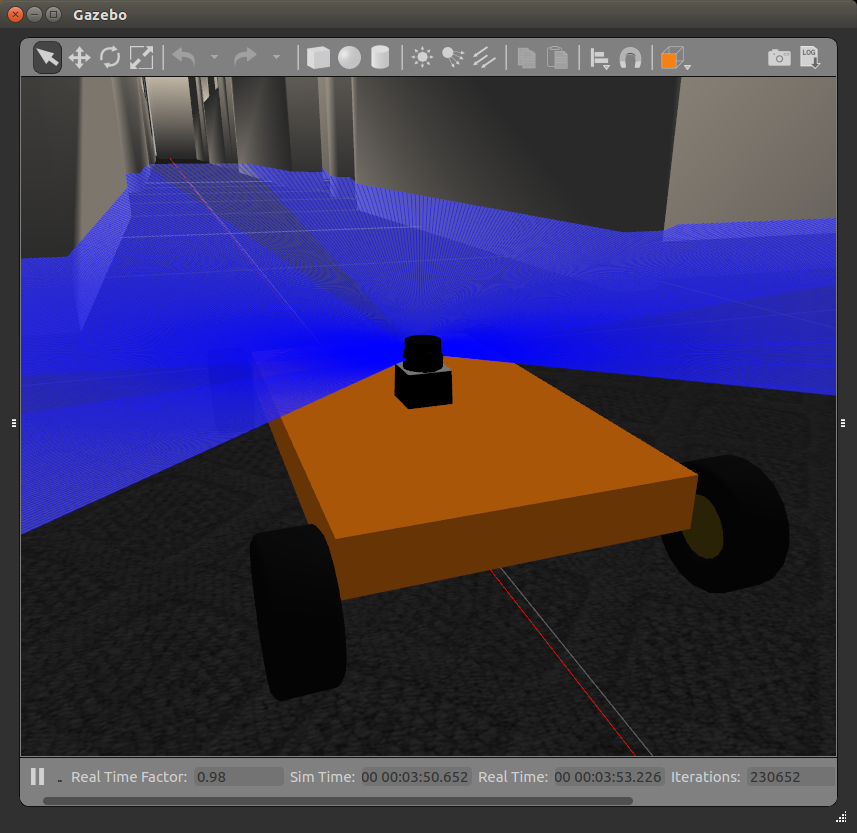
\includegraphics[width=\textwidth]{qbot-gazebo}
    \label{fig:gaz}
    \caption{Robot with laser sensor in Gazebo}
  \end{subfigure}
  \begin{subfigure}[b]{0.48\textwidth}
    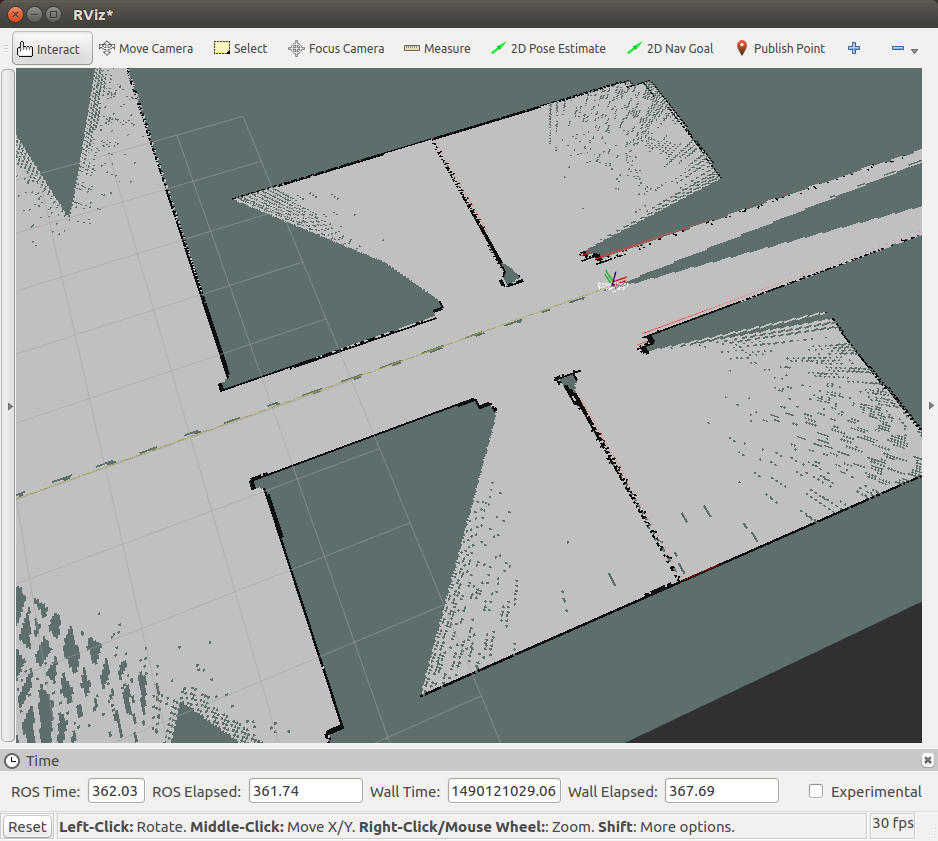
\includegraphics[width=\textwidth]{qbot-rviz}
    \label{fig:rviz}
    \caption{Already mapped environment in Rviz}
  \end{subfigure}
  \caption{Simulation of four-wheeled robot with SLAM and navigation}
  \label{fig:gaz-rviz}
\end{figure}
Here I only provide small code snippets. You can find the full package
on \url{https://github.com/zwilling/4-wheeled-ros-robot} with some
instructions how to run it. I also provided a demo video
here: \url{https://youtu.be/NZH0TxBaLyU}\\When you try it out yourself, don't expect too much from
the simulation because the skid-steering is
inaccurately simulated. However this could be fixed by tuning physics parameters
in the simulation or by simulating the robot motion on a higher abstraction
level.

As ROS-based mapping system, I utilize \texttt{gmapping}. It builds a map and
localizes the robot in it. It depends on laser data generated by a
simulated Hokuyo sensor and on the odometry of the robot, which is
provided by the \texttt{gazebo\_ros\_skid\_steer\_drive} plugin for
Gazebo. This plugin also applies velocity commands to the simulated
wheels. \texttt{gmapping} can be started with the ros launch file
shown in~\reflst{lst:gmapping}
\begin{figure}
\begin{lstlisting}[showlines,language=XML, caption={Launch file for \texttt{gmapping}},
    label=lst:gmapping]
<launch>
  <node pkg="tf" type="static_transform_publisher" name="hokuyo_link_broadcaster"
        args="0 0 0.08 0 0 0 1 base_link base_laser 100" />
  <node pkg="gmapping" type="slam_gmapping" name="slam_gmapping" output="screen">
    <rosparam>
      odom_frame: odom
      map_update_interval: 1.0
      maxUrange: 10.0
      base_frame: base_link
      [...]
    </rosparam>
    <remap from="/scan" to="/qbot/laser/scan" />
  </node>
</launch>
\end{lstlisting}
\end{figure}


\section{Navigation}
\label{sec:e5}
\textbf{Task:} Demonstrate via ROS libraries and C++ code, how the
outputs of the mapping system could be broadcasted and subsequently
utilised to navigate the robot to desired locations in Cartesian/world
coordinates.\\
\vspace{0.2cm}\\
The \texttt{gmapping} package used in the previous section
periodically publishes the transform between the robot and the map
frame and the updated map on the \texttt{/map} topic. This can be used
in conjunction with the laser data and the velocity controller to
navigate the robot around with collision avoidance. A ROS package
providing this is \texttt{move\_base}. It generates costmaps from map
and laser data and handles motion planning to navigate to a goal
specified on the \texttt{/move\_base\_simple/goal} topic. The node
that needs to be added to the launch file is shown
in~\reflst{lst:move-base}.
\begin{figure}
\begin{lstlisting}[showlines,language=XML,
    caption={\texttt{move\_base} node for the navigation launch file},
    label=lst:move-base]
  <node pkg="move_base" type="move_base" respawn="false" name="move_base" output="screen">
    <rosparam file="params/costmap_common.yaml" command="load" ns="global_costmap" />
    <rosparam file="params/costmap_common.yaml" command="load" ns="local_costmap" />
    <rosparam file="params/local_costmap.yaml" command="load" />
    <rosparam file="params/global_costmap.yaml" command="load" />
    <rosparam file="params/base_local_planner.yaml" command="load" />
    <remap from="/cmd_vel" to="/qbot/cmd_vel" />
  </node>
\end{lstlisting}
\end{figure}
There are multiple configuration files specifying collision avoidance
parameters and locomotion capabilities of the robot.


\section{ROS-based Graphical User Interface}
\label{sec:e6}
\begin{wrapfigure}{r}{0.4\textwidth}
  \centering
  \vspace{-0.4cm}
  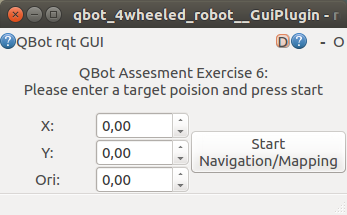
\includegraphics[width=0.4\textwidth]{qbot-gui}
  \caption{\texttt{rqt} plugin to send navigation commands}
  \label{fig:rqt}
  \vspace{-0.4cm}
\end{wrapfigure}
\textbf{Task:} Append a button/checkbox to a custom ROS-based
graphical user interface, whose toggling/checking activates the
previously-designed controller (C++ code).\\
\vspace{0.2cm}\\
This task is solved with a C++ \texttt{rqt} plugin, which is shown
in~\reffig{fig:rqt}.
This GUI plugin can be added to a \texttt{rqt} window and sends a
\texttt{geometry\_msgs::PoseStamped} message on the
\texttt{/move\_base\_simple/goal} topic to start the navigation. The
target coordinates and orientation are read from the corresponding
fields in the GUI. \reflst{lst:gui} shows how this message is sent in
the callback function of the button being pressed.
\begin{figure}
\begin{lstlisting}[showlines,style=SmallCpp, caption={\texttt{rqt}
        function starting the navigation},
    label=lst:gui]
void GuiPlugin::on_start_button_push()
{
  //button was pushed
  //build navigation goal message from values in SpinBoxes
  geometry_msgs::PoseStamped msg;
  msg.pose.position.x = ui_.doubleSpinBox_x->value();
  msg.pose.position.y = ui_.doubleSpinBox_y->value();
  //get Quaternion from yaw to write it into the msg
  tf::Quaternion q;
  q.setRPY(0.0 , 0.0, ui_.doubleSpinBox_ori->value());
  tf::quaternionTFToMsg(q, msg.pose.orientation);
  msg.header.frame_id = "map";
  msg.header.stamp = ros::Time::now();

  //send
  navigation_pub_.publish(msg);
}
\end{lstlisting}
\end{figure}


\bibliographystyle{apalike}
\bibliography{references}

\end{document}
